% Figure 1 d'A1 — GENEREE par analyses/p717_figure_gyra94.py (P7.17), ne pas editer a la main.
% Sources : WHO-UCN-TB-2023.7-eng_genomic_coordinates.txt, NC_000962.3.fasta, p77_C1_residuel.tsv.
\documentclass[border=3pt]{standalone}
\usepackage[T1]{fontenc}
\usepackage[utf8]{inputenc}
\usepackage{tikz}
\usetikzlibrary{decorations.pathreplacing}
\definecolor{refcol}{HTML}{595959}
\definecolor{codon94col}{HTML}{0072B2}
\definecolor{codon95col}{HTML}{7B52AB}
\definecolor{appelcol}{HTML}{E69F00}
\definecolor{listecol}{HTML}{0072B2}
\definecolor{combinecol}{HTML}{009E73}
\definecolor{absentcol}{HTML}{D55E00}
\begin{document}
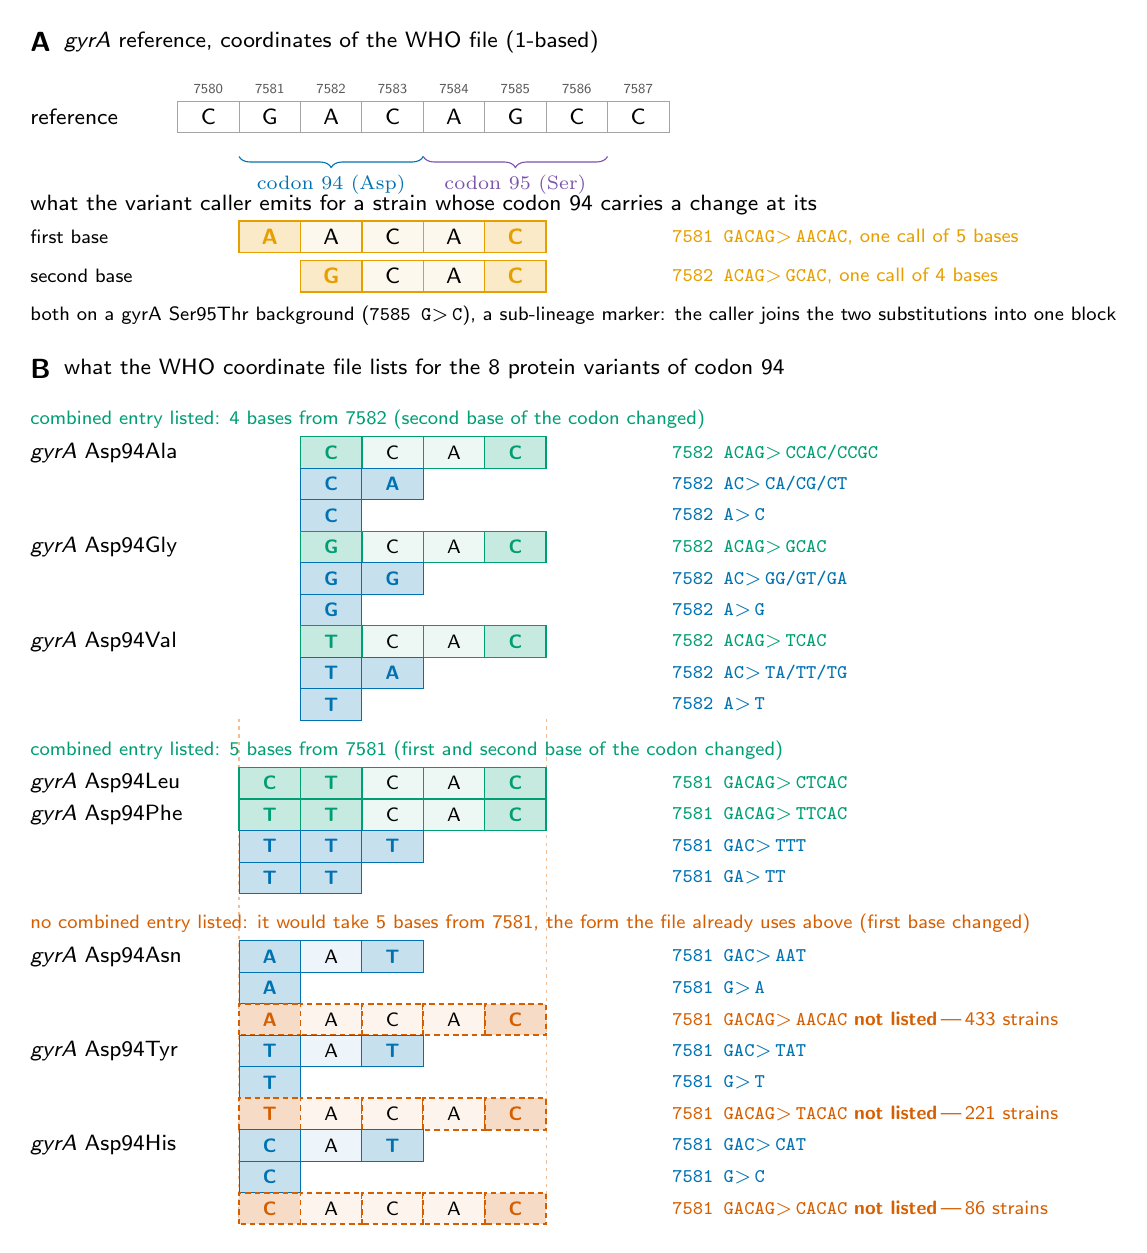
\begin{tikzpicture}[x=1cm,y=1cm,font=\sffamily]
  \node[anchor=west,inner sep=1pt] at (-2.301,0.000) {\normalsize \textbf{A}};
  \node[anchor=west,inner sep=1pt] at (-1.872,0.000) {\footnotesize \textit{gyrA} reference, coordinates of the WHO file (1-based)};
  \node[anchor=center,text={refcol},inner sep=1pt] at (0.000,-0.600) {\tiny 7580};
  \node[anchor=center,text={refcol},inner sep=1pt] at (0.780,-0.600) {\tiny 7581};
  \node[anchor=center,text={refcol},inner sep=1pt] at (1.560,-0.600) {\tiny 7582};
  \node[anchor=center,text={refcol},inner sep=1pt] at (2.340,-0.600) {\tiny 7583};
  \node[anchor=center,text={refcol},inner sep=1pt] at (3.120,-0.600) {\tiny 7584};
  \node[anchor=center,text={refcol},inner sep=1pt] at (3.900,-0.600) {\tiny 7585};
  \node[anchor=center,text={refcol},inner sep=1pt] at (4.680,-0.600) {\tiny 7586};
  \node[anchor=center,text={refcol},inner sep=1pt] at (5.460,-0.600) {\tiny 7587};
  \draw[draw=refcol!55,line width=0.3pt,fill=none] (-0.390,-1.160) rectangle (0.390,-0.760);
  \node[anchor=center,inner sep=0pt] at (0.000,-0.960) {\footnotesize C};
  \draw[draw=refcol!55,line width=0.3pt,fill=none] (0.390,-1.160) rectangle (1.170,-0.760);
  \node[anchor=center,inner sep=0pt] at (0.780,-0.960) {\footnotesize G};
  \draw[draw=refcol!55,line width=0.3pt,fill=none] (1.170,-1.160) rectangle (1.950,-0.760);
  \node[anchor=center,inner sep=0pt] at (1.560,-0.960) {\footnotesize A};
  \draw[draw=refcol!55,line width=0.3pt,fill=none] (1.950,-1.160) rectangle (2.730,-0.760);
  \node[anchor=center,inner sep=0pt] at (2.340,-0.960) {\footnotesize C};
  \draw[draw=refcol!55,line width=0.3pt,fill=none] (2.730,-1.160) rectangle (3.510,-0.760);
  \node[anchor=center,inner sep=0pt] at (3.120,-0.960) {\footnotesize A};
  \draw[draw=refcol!55,line width=0.3pt,fill=none] (3.510,-1.160) rectangle (4.290,-0.760);
  \node[anchor=center,inner sep=0pt] at (3.900,-0.960) {\footnotesize G};
  \draw[draw=refcol!55,line width=0.3pt,fill=none] (4.290,-1.160) rectangle (5.070,-0.760);
  \node[anchor=center,inner sep=0pt] at (4.680,-0.960) {\footnotesize C};
  \draw[draw=refcol!55,line width=0.3pt,fill=none] (5.070,-1.160) rectangle (5.850,-0.760);
  \node[anchor=center,inner sep=0pt] at (5.460,-0.960) {\footnotesize C};
  \node[anchor=west,inner sep=1pt] at (-2.301,-0.960) {\footnotesize reference};
  \draw[decorate,decoration={brace,mirror,amplitude=4pt},codon94col] (0.390,-1.460) -- (2.730,-1.460) node[midway,below=3pt,font=\scriptsize,text={codon94col}] {codon 94 (Asp)};
  \draw[decorate,decoration={brace,mirror,amplitude=4pt},codon95col] (2.730,-1.460) -- (5.070,-1.460) node[midway,below=3pt,font=\scriptsize,text={codon95col}] {codon 95 (Ser)};
  \node[anchor=west,inner sep=1pt] at (-2.301,-2.080) {\footnotesize what the variant caller emits for a strain whose codon 94 carries a change at its};
  \draw[draw=appelcol,line width=0.5pt,fill=appelcol!22] (0.390,-2.680) rectangle (1.170,-2.280);
  \node[anchor=center,text={appelcol},inner sep=0pt] at (0.780,-2.480) {\footnotesize \textbf{A}};
  \draw[draw=appelcol,line width=0.5pt,fill=appelcol!7] (1.170,-2.680) rectangle (1.950,-2.280);
  \node[anchor=center,inner sep=0pt] at (1.560,-2.480) {\footnotesize A};
  \draw[draw=appelcol,line width=0.5pt,fill=appelcol!7] (1.950,-2.680) rectangle (2.730,-2.280);
  \node[anchor=center,inner sep=0pt] at (2.340,-2.480) {\footnotesize C};
  \draw[draw=appelcol,line width=0.5pt,fill=appelcol!7] (2.730,-2.680) rectangle (3.510,-2.280);
  \node[anchor=center,inner sep=0pt] at (3.120,-2.480) {\footnotesize A};
  \draw[draw=appelcol,line width=0.5pt,fill=appelcol!22] (3.510,-2.680) rectangle (4.290,-2.280);
  \node[anchor=center,text={appelcol},inner sep=0pt] at (3.900,-2.480) {\footnotesize \textbf{C}};
  \node[anchor=west,inner sep=1pt] at (-2.301,-2.480) {\scriptsize first base};
  \node[anchor=west,text={appelcol},inner sep=1pt] at (5.850,-2.480) {\scriptsize \texttt{7581 GACAG$>$\,AACAC}, one call of 5 bases};
  \draw[draw=appelcol,line width=0.5pt,fill=appelcol!22] (1.170,-3.180) rectangle (1.950,-2.780);
  \node[anchor=center,text={appelcol},inner sep=0pt] at (1.560,-2.980) {\footnotesize \textbf{G}};
  \draw[draw=appelcol,line width=0.5pt,fill=appelcol!7] (1.950,-3.180) rectangle (2.730,-2.780);
  \node[anchor=center,inner sep=0pt] at (2.340,-2.980) {\footnotesize C};
  \draw[draw=appelcol,line width=0.5pt,fill=appelcol!7] (2.730,-3.180) rectangle (3.510,-2.780);
  \node[anchor=center,inner sep=0pt] at (3.120,-2.980) {\footnotesize A};
  \draw[draw=appelcol,line width=0.5pt,fill=appelcol!22] (3.510,-3.180) rectangle (4.290,-2.780);
  \node[anchor=center,text={appelcol},inner sep=0pt] at (3.900,-2.980) {\footnotesize \textbf{C}};
  \node[anchor=west,inner sep=1pt] at (-2.301,-2.980) {\scriptsize second base};
  \node[anchor=west,text={appelcol},inner sep=1pt] at (5.850,-2.980) {\scriptsize \texttt{7582 ACAG$>$\,GCAC}, one call of 4 bases};
  \node[anchor=west,inner sep=1pt] at (-2.301,-3.480) {\scriptsize both on a gyrA Ser95Thr background (\texttt{7585 G$>$\,C}), a sub-lineage marker: the caller joins the two substitutions into one block};
  \node[anchor=west,inner sep=1pt] at (-2.301,-4.160) {\normalsize \textbf{B}};
  \node[anchor=west,inner sep=1pt] at (-1.872,-4.160) {\footnotesize what the WHO coordinate file lists for the 8 protein variants of codon 94};
  \node[anchor=west,text={combinecol},inner sep=1pt] at (-2.301,-4.800) {\scriptsize combined entry listed: 4 bases from 7582 (second base of the codon changed)};
  \draw[draw=combinecol,line width=0.5pt,fill=combinecol!22] (1.170,-5.420) rectangle (1.950,-5.020);
  \node[anchor=center,text={combinecol},inner sep=0pt] at (1.560,-5.220) {\scriptsize \textbf{C}};
  \draw[draw=combinecol,line width=0.5pt,fill=combinecol!7] (1.950,-5.420) rectangle (2.730,-5.020);
  \node[anchor=center,inner sep=0pt] at (2.340,-5.220) {\scriptsize C};
  \draw[draw=combinecol,line width=0.5pt,fill=combinecol!7] (2.730,-5.420) rectangle (3.510,-5.020);
  \node[anchor=center,inner sep=0pt] at (3.120,-5.220) {\scriptsize A};
  \draw[draw=combinecol,line width=0.5pt,fill=combinecol!22] (3.510,-5.420) rectangle (4.290,-5.020);
  \node[anchor=center,text={combinecol},inner sep=0pt] at (3.900,-5.220) {\scriptsize \textbf{C}};
  \node[anchor=west,text={combinecol},inner sep=1pt] at (5.850,-5.220) {\scriptsize \texttt{7582 ACAG$>$\,CCAC/CCGC}};
  \draw[draw=listecol,line width=0.3pt,fill=listecol!22] (1.170,-5.820) rectangle (1.950,-5.420);
  \node[anchor=center,text={listecol},inner sep=0pt] at (1.560,-5.620) {\scriptsize \textbf{C}};
  \draw[draw=listecol,line width=0.3pt,fill=listecol!22] (1.950,-5.820) rectangle (2.730,-5.420);
  \node[anchor=center,text={listecol},inner sep=0pt] at (2.340,-5.620) {\scriptsize \textbf{A}};
  \node[anchor=west,text={listecol},inner sep=1pt] at (5.850,-5.620) {\scriptsize \texttt{7582 AC$>$\,CA/CG/CT}};
  \draw[draw=listecol,line width=0.3pt,fill=listecol!22] (1.170,-6.220) rectangle (1.950,-5.820);
  \node[anchor=center,text={listecol},inner sep=0pt] at (1.560,-6.020) {\scriptsize \textbf{C}};
  \node[anchor=west,text={listecol},inner sep=1pt] at (5.850,-6.020) {\scriptsize \texttt{7582 A$>$\,C}};
  \node[anchor=west,inner sep=1pt] at (-2.301,-5.220) {\footnotesize \textit{gyrA} Asp94Ala};
  \draw[draw=combinecol,line width=0.5pt,fill=combinecol!22] (1.170,-6.620) rectangle (1.950,-6.220);
  \node[anchor=center,text={combinecol},inner sep=0pt] at (1.560,-6.420) {\scriptsize \textbf{G}};
  \draw[draw=combinecol,line width=0.5pt,fill=combinecol!7] (1.950,-6.620) rectangle (2.730,-6.220);
  \node[anchor=center,inner sep=0pt] at (2.340,-6.420) {\scriptsize C};
  \draw[draw=combinecol,line width=0.5pt,fill=combinecol!7] (2.730,-6.620) rectangle (3.510,-6.220);
  \node[anchor=center,inner sep=0pt] at (3.120,-6.420) {\scriptsize A};
  \draw[draw=combinecol,line width=0.5pt,fill=combinecol!22] (3.510,-6.620) rectangle (4.290,-6.220);
  \node[anchor=center,text={combinecol},inner sep=0pt] at (3.900,-6.420) {\scriptsize \textbf{C}};
  \node[anchor=west,text={combinecol},inner sep=1pt] at (5.850,-6.420) {\scriptsize \texttt{7582 ACAG$>$\,GCAC}};
  \draw[draw=listecol,line width=0.3pt,fill=listecol!22] (1.170,-7.020) rectangle (1.950,-6.620);
  \node[anchor=center,text={listecol},inner sep=0pt] at (1.560,-6.820) {\scriptsize \textbf{G}};
  \draw[draw=listecol,line width=0.3pt,fill=listecol!22] (1.950,-7.020) rectangle (2.730,-6.620);
  \node[anchor=center,text={listecol},inner sep=0pt] at (2.340,-6.820) {\scriptsize \textbf{G}};
  \node[anchor=west,text={listecol},inner sep=1pt] at (5.850,-6.820) {\scriptsize \texttt{7582 AC$>$\,GG/GT/GA}};
  \draw[draw=listecol,line width=0.3pt,fill=listecol!22] (1.170,-7.420) rectangle (1.950,-7.020);
  \node[anchor=center,text={listecol},inner sep=0pt] at (1.560,-7.220) {\scriptsize \textbf{G}};
  \node[anchor=west,text={listecol},inner sep=1pt] at (5.850,-7.220) {\scriptsize \texttt{7582 A$>$\,G}};
  \node[anchor=west,inner sep=1pt] at (-2.301,-6.420) {\footnotesize \textit{gyrA} Asp94Gly};
  \draw[draw=combinecol,line width=0.5pt,fill=combinecol!22] (1.170,-7.820) rectangle (1.950,-7.420);
  \node[anchor=center,text={combinecol},inner sep=0pt] at (1.560,-7.620) {\scriptsize \textbf{T}};
  \draw[draw=combinecol,line width=0.5pt,fill=combinecol!7] (1.950,-7.820) rectangle (2.730,-7.420);
  \node[anchor=center,inner sep=0pt] at (2.340,-7.620) {\scriptsize C};
  \draw[draw=combinecol,line width=0.5pt,fill=combinecol!7] (2.730,-7.820) rectangle (3.510,-7.420);
  \node[anchor=center,inner sep=0pt] at (3.120,-7.620) {\scriptsize A};
  \draw[draw=combinecol,line width=0.5pt,fill=combinecol!22] (3.510,-7.820) rectangle (4.290,-7.420);
  \node[anchor=center,text={combinecol},inner sep=0pt] at (3.900,-7.620) {\scriptsize \textbf{C}};
  \node[anchor=west,text={combinecol},inner sep=1pt] at (5.850,-7.620) {\scriptsize \texttt{7582 ACAG$>$\,TCAC}};
  \draw[draw=listecol,line width=0.3pt,fill=listecol!22] (1.170,-8.220) rectangle (1.950,-7.820);
  \node[anchor=center,text={listecol},inner sep=0pt] at (1.560,-8.020) {\scriptsize \textbf{T}};
  \draw[draw=listecol,line width=0.3pt,fill=listecol!22] (1.950,-8.220) rectangle (2.730,-7.820);
  \node[anchor=center,text={listecol},inner sep=0pt] at (2.340,-8.020) {\scriptsize \textbf{A}};
  \node[anchor=west,text={listecol},inner sep=1pt] at (5.850,-8.020) {\scriptsize \texttt{7582 AC$>$\,TA/TT/TG}};
  \draw[draw=listecol,line width=0.3pt,fill=listecol!22] (1.170,-8.620) rectangle (1.950,-8.220);
  \node[anchor=center,text={listecol},inner sep=0pt] at (1.560,-8.420) {\scriptsize \textbf{T}};
  \node[anchor=west,text={listecol},inner sep=1pt] at (5.850,-8.420) {\scriptsize \texttt{7582 A$>$\,T}};
  \node[anchor=west,inner sep=1pt] at (-2.301,-7.620) {\footnotesize \textit{gyrA} Asp94Val};
  \draw[absentcol!40,line width=0.4pt,dash pattern=on 1.2pt off 1.6pt] (0.390,-8.600) -- (0.390,-15.020);
  \draw[absentcol!40,line width=0.4pt,dash pattern=on 1.2pt off 1.6pt] (4.290,-8.600) -- (4.290,-15.020);
  \node[anchor=west,text={combinecol},inner sep=1pt] at (-2.301,-9.000) {\scriptsize combined entry listed: 5 bases from 7581 (first and second base of the codon changed)};
  \draw[draw=combinecol,line width=0.5pt,fill=combinecol!22] (0.390,-9.620) rectangle (1.170,-9.220);
  \node[anchor=center,text={combinecol},inner sep=0pt] at (0.780,-9.420) {\scriptsize \textbf{C}};
  \draw[draw=combinecol,line width=0.5pt,fill=combinecol!22] (1.170,-9.620) rectangle (1.950,-9.220);
  \node[anchor=center,text={combinecol},inner sep=0pt] at (1.560,-9.420) {\scriptsize \textbf{T}};
  \draw[draw=combinecol,line width=0.5pt,fill=combinecol!7] (1.950,-9.620) rectangle (2.730,-9.220);
  \node[anchor=center,inner sep=0pt] at (2.340,-9.420) {\scriptsize C};
  \draw[draw=combinecol,line width=0.5pt,fill=combinecol!7] (2.730,-9.620) rectangle (3.510,-9.220);
  \node[anchor=center,inner sep=0pt] at (3.120,-9.420) {\scriptsize A};
  \draw[draw=combinecol,line width=0.5pt,fill=combinecol!22] (3.510,-9.620) rectangle (4.290,-9.220);
  \node[anchor=center,text={combinecol},inner sep=0pt] at (3.900,-9.420) {\scriptsize \textbf{C}};
  \node[anchor=west,text={combinecol},inner sep=1pt] at (5.850,-9.420) {\scriptsize \texttt{7581 GACAG$>$\,CTCAC}};
  \node[anchor=west,inner sep=1pt] at (-2.301,-9.420) {\footnotesize \textit{gyrA} Asp94Leu};
  \draw[draw=combinecol,line width=0.5pt,fill=combinecol!22] (0.390,-10.020) rectangle (1.170,-9.620);
  \node[anchor=center,text={combinecol},inner sep=0pt] at (0.780,-9.820) {\scriptsize \textbf{T}};
  \draw[draw=combinecol,line width=0.5pt,fill=combinecol!22] (1.170,-10.020) rectangle (1.950,-9.620);
  \node[anchor=center,text={combinecol},inner sep=0pt] at (1.560,-9.820) {\scriptsize \textbf{T}};
  \draw[draw=combinecol,line width=0.5pt,fill=combinecol!7] (1.950,-10.020) rectangle (2.730,-9.620);
  \node[anchor=center,inner sep=0pt] at (2.340,-9.820) {\scriptsize C};
  \draw[draw=combinecol,line width=0.5pt,fill=combinecol!7] (2.730,-10.020) rectangle (3.510,-9.620);
  \node[anchor=center,inner sep=0pt] at (3.120,-9.820) {\scriptsize A};
  \draw[draw=combinecol,line width=0.5pt,fill=combinecol!22] (3.510,-10.020) rectangle (4.290,-9.620);
  \node[anchor=center,text={combinecol},inner sep=0pt] at (3.900,-9.820) {\scriptsize \textbf{C}};
  \node[anchor=west,text={combinecol},inner sep=1pt] at (5.850,-9.820) {\scriptsize \texttt{7581 GACAG$>$\,TTCAC}};
  \draw[draw=listecol,line width=0.3pt,fill=listecol!22] (0.390,-10.420) rectangle (1.170,-10.020);
  \node[anchor=center,text={listecol},inner sep=0pt] at (0.780,-10.220) {\scriptsize \textbf{T}};
  \draw[draw=listecol,line width=0.3pt,fill=listecol!22] (1.170,-10.420) rectangle (1.950,-10.020);
  \node[anchor=center,text={listecol},inner sep=0pt] at (1.560,-10.220) {\scriptsize \textbf{T}};
  \draw[draw=listecol,line width=0.3pt,fill=listecol!22] (1.950,-10.420) rectangle (2.730,-10.020);
  \node[anchor=center,text={listecol},inner sep=0pt] at (2.340,-10.220) {\scriptsize \textbf{T}};
  \node[anchor=west,text={listecol},inner sep=1pt] at (5.850,-10.220) {\scriptsize \texttt{7581 GAC$>$\,TTT}};
  \draw[draw=listecol,line width=0.3pt,fill=listecol!22] (0.390,-10.820) rectangle (1.170,-10.420);
  \node[anchor=center,text={listecol},inner sep=0pt] at (0.780,-10.620) {\scriptsize \textbf{T}};
  \draw[draw=listecol,line width=0.3pt,fill=listecol!22] (1.170,-10.820) rectangle (1.950,-10.420);
  \node[anchor=center,text={listecol},inner sep=0pt] at (1.560,-10.620) {\scriptsize \textbf{T}};
  \node[anchor=west,text={listecol},inner sep=1pt] at (5.850,-10.620) {\scriptsize \texttt{7581 GA$>$\,TT}};
  \node[anchor=west,inner sep=1pt] at (-2.301,-9.820) {\footnotesize \textit{gyrA} Asp94Phe};
  \node[anchor=west,text={absentcol},inner sep=1pt] at (-2.301,-11.200) {\scriptsize no combined entry listed: it would take 5 bases from 7581, the form the file already uses above (first base changed)};
  \draw[draw=listecol,line width=0.3pt,fill=listecol!22] (0.390,-11.820) rectangle (1.170,-11.420);
  \node[anchor=center,text={listecol},inner sep=0pt] at (0.780,-11.620) {\scriptsize \textbf{A}};
  \draw[draw=listecol,line width=0.3pt,fill=listecol!7] (1.170,-11.820) rectangle (1.950,-11.420);
  \node[anchor=center,inner sep=0pt] at (1.560,-11.620) {\scriptsize A};
  \draw[draw=listecol,line width=0.3pt,fill=listecol!22] (1.950,-11.820) rectangle (2.730,-11.420);
  \node[anchor=center,text={listecol},inner sep=0pt] at (2.340,-11.620) {\scriptsize \textbf{T}};
  \node[anchor=west,text={listecol},inner sep=1pt] at (5.850,-11.620) {\scriptsize \texttt{7581 GAC$>$\,AAT}};
  \draw[draw=listecol,line width=0.3pt,fill=listecol!22] (0.390,-12.220) rectangle (1.170,-11.820);
  \node[anchor=center,text={listecol},inner sep=0pt] at (0.780,-12.020) {\scriptsize \textbf{A}};
  \node[anchor=west,text={listecol},inner sep=1pt] at (5.850,-12.020) {\scriptsize \texttt{7581 G$>$\,A}};
  \draw[draw=absentcol,line width=0.6pt,dash pattern=on 2pt off 1.4pt,fill=absentcol!22] (0.390,-12.620) rectangle (1.170,-12.220);
  \node[anchor=center,text={absentcol},inner sep=0pt] at (0.780,-12.420) {\scriptsize \textbf{A}};
  \draw[draw=absentcol,line width=0.6pt,dash pattern=on 2pt off 1.4pt,fill=absentcol!7] (1.170,-12.620) rectangle (1.950,-12.220);
  \node[anchor=center,inner sep=0pt] at (1.560,-12.420) {\scriptsize A};
  \draw[draw=absentcol,line width=0.6pt,dash pattern=on 2pt off 1.4pt,fill=absentcol!7] (1.950,-12.620) rectangle (2.730,-12.220);
  \node[anchor=center,inner sep=0pt] at (2.340,-12.420) {\scriptsize C};
  \draw[draw=absentcol,line width=0.6pt,dash pattern=on 2pt off 1.4pt,fill=absentcol!7] (2.730,-12.620) rectangle (3.510,-12.220);
  \node[anchor=center,inner sep=0pt] at (3.120,-12.420) {\scriptsize A};
  \draw[draw=absentcol,line width=0.6pt,dash pattern=on 2pt off 1.4pt,fill=absentcol!22] (3.510,-12.620) rectangle (4.290,-12.220);
  \node[anchor=center,text={absentcol},inner sep=0pt] at (3.900,-12.420) {\scriptsize \textbf{C}};
  \node[anchor=west,text={absentcol},inner sep=1pt] at (5.850,-12.420) {\scriptsize \texttt{7581 GACAG$>$\,AACAC} \textbf{not listed}\,\textemdash\,433 strains};
  \node[anchor=west,inner sep=1pt] at (-2.301,-11.620) {\footnotesize \textit{gyrA} Asp94Asn};
  \draw[draw=listecol,line width=0.3pt,fill=listecol!22] (0.390,-13.020) rectangle (1.170,-12.620);
  \node[anchor=center,text={listecol},inner sep=0pt] at (0.780,-12.820) {\scriptsize \textbf{T}};
  \draw[draw=listecol,line width=0.3pt,fill=listecol!7] (1.170,-13.020) rectangle (1.950,-12.620);
  \node[anchor=center,inner sep=0pt] at (1.560,-12.820) {\scriptsize A};
  \draw[draw=listecol,line width=0.3pt,fill=listecol!22] (1.950,-13.020) rectangle (2.730,-12.620);
  \node[anchor=center,text={listecol},inner sep=0pt] at (2.340,-12.820) {\scriptsize \textbf{T}};
  \node[anchor=west,text={listecol},inner sep=1pt] at (5.850,-12.820) {\scriptsize \texttt{7581 GAC$>$\,TAT}};
  \draw[draw=listecol,line width=0.3pt,fill=listecol!22] (0.390,-13.420) rectangle (1.170,-13.020);
  \node[anchor=center,text={listecol},inner sep=0pt] at (0.780,-13.220) {\scriptsize \textbf{T}};
  \node[anchor=west,text={listecol},inner sep=1pt] at (5.850,-13.220) {\scriptsize \texttt{7581 G$>$\,T}};
  \draw[draw=absentcol,line width=0.6pt,dash pattern=on 2pt off 1.4pt,fill=absentcol!22] (0.390,-13.820) rectangle (1.170,-13.420);
  \node[anchor=center,text={absentcol},inner sep=0pt] at (0.780,-13.620) {\scriptsize \textbf{T}};
  \draw[draw=absentcol,line width=0.6pt,dash pattern=on 2pt off 1.4pt,fill=absentcol!7] (1.170,-13.820) rectangle (1.950,-13.420);
  \node[anchor=center,inner sep=0pt] at (1.560,-13.620) {\scriptsize A};
  \draw[draw=absentcol,line width=0.6pt,dash pattern=on 2pt off 1.4pt,fill=absentcol!7] (1.950,-13.820) rectangle (2.730,-13.420);
  \node[anchor=center,inner sep=0pt] at (2.340,-13.620) {\scriptsize C};
  \draw[draw=absentcol,line width=0.6pt,dash pattern=on 2pt off 1.4pt,fill=absentcol!7] (2.730,-13.820) rectangle (3.510,-13.420);
  \node[anchor=center,inner sep=0pt] at (3.120,-13.620) {\scriptsize A};
  \draw[draw=absentcol,line width=0.6pt,dash pattern=on 2pt off 1.4pt,fill=absentcol!22] (3.510,-13.820) rectangle (4.290,-13.420);
  \node[anchor=center,text={absentcol},inner sep=0pt] at (3.900,-13.620) {\scriptsize \textbf{C}};
  \node[anchor=west,text={absentcol},inner sep=1pt] at (5.850,-13.620) {\scriptsize \texttt{7581 GACAG$>$\,TACAC} \textbf{not listed}\,\textemdash\,221 strains};
  \node[anchor=west,inner sep=1pt] at (-2.301,-12.820) {\footnotesize \textit{gyrA} Asp94Tyr};
  \draw[draw=listecol,line width=0.3pt,fill=listecol!22] (0.390,-14.220) rectangle (1.170,-13.820);
  \node[anchor=center,text={listecol},inner sep=0pt] at (0.780,-14.020) {\scriptsize \textbf{C}};
  \draw[draw=listecol,line width=0.3pt,fill=listecol!7] (1.170,-14.220) rectangle (1.950,-13.820);
  \node[anchor=center,inner sep=0pt] at (1.560,-14.020) {\scriptsize A};
  \draw[draw=listecol,line width=0.3pt,fill=listecol!22] (1.950,-14.220) rectangle (2.730,-13.820);
  \node[anchor=center,text={listecol},inner sep=0pt] at (2.340,-14.020) {\scriptsize \textbf{T}};
  \node[anchor=west,text={listecol},inner sep=1pt] at (5.850,-14.020) {\scriptsize \texttt{7581 GAC$>$\,CAT}};
  \draw[draw=listecol,line width=0.3pt,fill=listecol!22] (0.390,-14.620) rectangle (1.170,-14.220);
  \node[anchor=center,text={listecol},inner sep=0pt] at (0.780,-14.420) {\scriptsize \textbf{C}};
  \node[anchor=west,text={listecol},inner sep=1pt] at (5.850,-14.420) {\scriptsize \texttt{7581 G$>$\,C}};
  \draw[draw=absentcol,line width=0.6pt,dash pattern=on 2pt off 1.4pt,fill=absentcol!22] (0.390,-15.020) rectangle (1.170,-14.620);
  \node[anchor=center,text={absentcol},inner sep=0pt] at (0.780,-14.820) {\scriptsize \textbf{C}};
  \draw[draw=absentcol,line width=0.6pt,dash pattern=on 2pt off 1.4pt,fill=absentcol!7] (1.170,-15.020) rectangle (1.950,-14.620);
  \node[anchor=center,inner sep=0pt] at (1.560,-14.820) {\scriptsize A};
  \draw[draw=absentcol,line width=0.6pt,dash pattern=on 2pt off 1.4pt,fill=absentcol!7] (1.950,-15.020) rectangle (2.730,-14.620);
  \node[anchor=center,inner sep=0pt] at (2.340,-14.820) {\scriptsize C};
  \draw[draw=absentcol,line width=0.6pt,dash pattern=on 2pt off 1.4pt,fill=absentcol!7] (2.730,-15.020) rectangle (3.510,-14.620);
  \node[anchor=center,inner sep=0pt] at (3.120,-14.820) {\scriptsize A};
  \draw[draw=absentcol,line width=0.6pt,dash pattern=on 2pt off 1.4pt,fill=absentcol!22] (3.510,-15.020) rectangle (4.290,-14.620);
  \node[anchor=center,text={absentcol},inner sep=0pt] at (3.900,-14.820) {\scriptsize \textbf{C}};
  \node[anchor=west,text={absentcol},inner sep=1pt] at (5.850,-14.820) {\scriptsize \texttt{7581 GACAG$>$\,CACAC} \textbf{not listed}\,\textemdash\,86 strains};
  \node[anchor=west,inner sep=1pt] at (-2.301,-14.020) {\footnotesize \textit{gyrA} Asp94His};
\end{tikzpicture}
\end{document}
